\documentclass[3p,review,12pt]{elsarticle}
\usepackage{lineno,hyperref,notoccite,etoolbox}
\modulolinenumbers[5]
\makeatletter
\def\ps@pprintTitle{%
	\let\@oddhead\@empty
	\let\@evenhead\@empty
	\def\@oddfoot{\centerline{\thepage}}%
	\let\@evenfoot\@oddfoot}
\makeatother
\usepackage{setspace}
\singlespacing
\usepackage{mathptmx}
\usepackage{float,wrapfig}
\newcommand{\vs}{\vspace{2mm}}
\begin{document}

\begin{frontmatter}
	\title{Computational Methods for Amorphous Semiconductor Devices}
	
	\author[boise]{Ember L. Sikorski}
	
	
	\address[boise]{Boise State University}
	
	\begin{abstract}
\begin{itemize}
	\item DOS
	\item structural modeling
\end{itemize}
	\end{abstract}
	
	
\end{frontmatter}

\section{Introduction}
\subsection{Why model amorphous semiconductors?}


\subsection{How can we model amorphous semiconductors?}
\begin{figure}[H]
	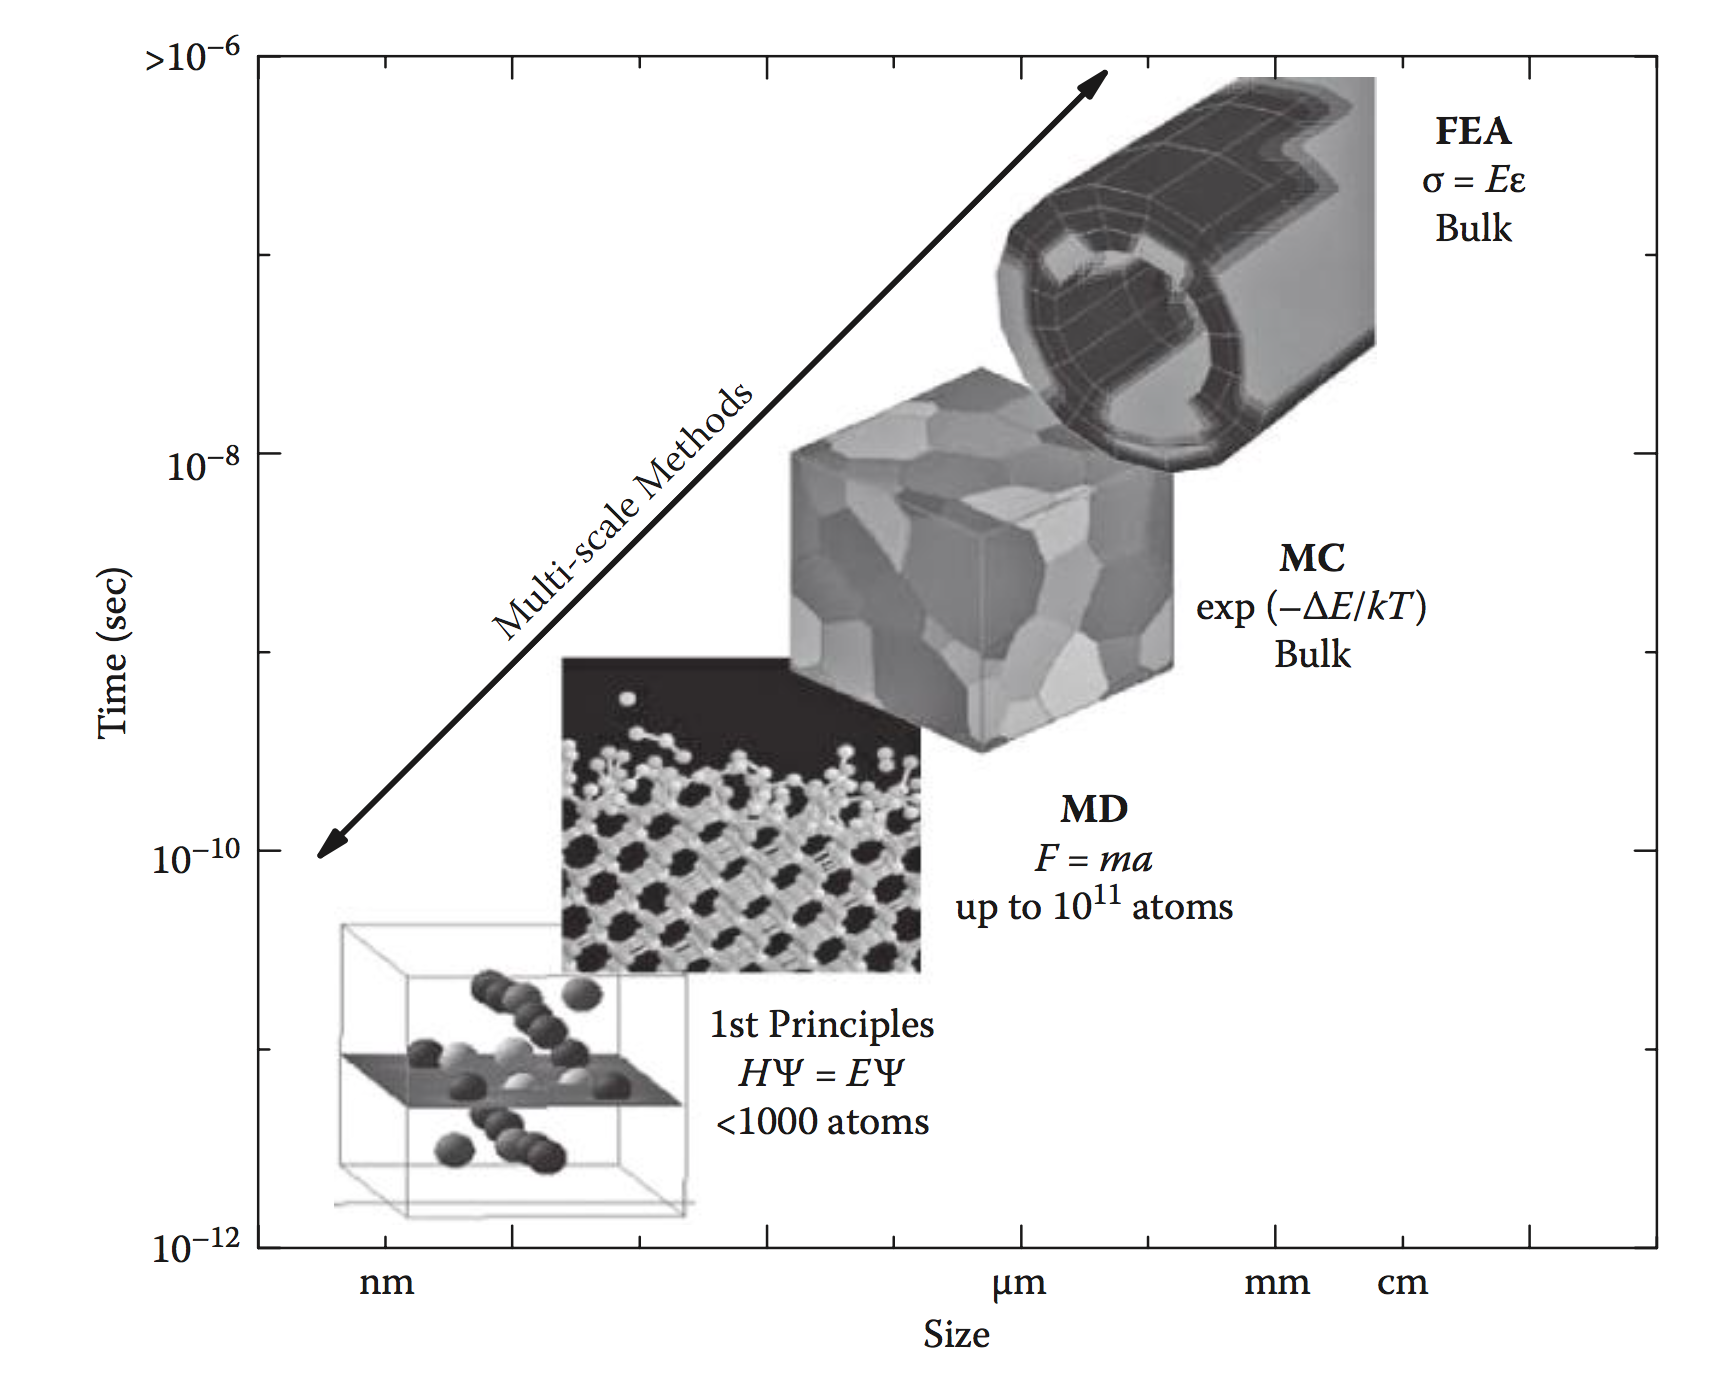
\includegraphics[width=\textwidth]{overview}
	\caption{Overview of computational methods with respect to time and size capabilities.}
\end{figure}


\section{Methods}


\subsection{Field Theory}

\subsection{Monte Carlo}

\subsection{Molecular Dynamics}

Molecular Dynamics (MD) is a classical method built off of

\begin{equation}
\vec{F}=m\vec{a} \qquad .
\end{equation}
Atoms are the smallest building block, represented as a sphere with a point mass \cite{Lee2012}. To calculate desired properties, atoms are allowed to ``relax" to their respective equilibrium distances, by moving down along the negative energy gradient:
\begin{equation}
\vec{F} = - \nabla U \qquad .
\end{equation}
A calculation begins with a set of starting atomic coordinates. The energy is calculated and the atoms are adjusted, following the gradient, to a more stable position. The energy is again calculated and compared to the previous step. This process continues until the differences between subsequent energy values reaches a predetermined stopping value, e.g. a difference of 1 $\times 10^-4$ eV or less.
\par
This method requires selection of so-called pair-potentials, which describe how atom $i$ interacts with atom $j$. The simplest potentail is the Lennard-Jones potential:

\begin{equation}
U_{ij}(r) = 4\epsilon \Bigg[\bigg(\frac{\sigma}{r}\bigg)^{12}-\bigg(\frac{\sigma}{r}\bigg)^{6}\Bigg] \qquad ,
\end{equation}
where $\epsilon$ is the depth of the energy well and $\sigma$ is the interatomic distance at which the potential is zero. However, this potential can only describe the interactions between atoms of the same element. In order to perform calculations on the majority of systems of interest, more complex pair-potentials are needed. Numerous potentials have been created, such as Embedded Atom Method (EAM) potentials which work for many metals and Tersoff potentials for covalent solids. 
\par 
An alternative method necessary for our discussion of AIMD in Section YYY is the Lagrangian:
\begin{equation}
L = K-U = \frac{1}{2}\sum_{i=1}^{3N}m_{i}v^{2}_{i}-U(r_{1}, \cdots, r_{3N})\qquad ,
\end{equation}
where $K$ is the kinetic energy, $U$ is the potential energy, and $N$ is the number of atoms.







\subsection{Density Functional Theory}
\begin{equation}
\hat{H}=-\frac{1}{2}\sum_{i}^{n}\nabla_{i}^{2}-\sum_{I}^{N}\sum_{i}^{n}\frac{Z_{I}}{|r_{Ii}|}+\sum_{i\neq j}^{n}\frac{1}{|r_{ij}|}
\end{equation}

\begin{equation}
\rho (r) = \sum_{i}|\phi _{i}(r)|^{2}
\end{equation}


\subsection{\emph{Ab intio} Molecular Dynamics}
\emph{Ab initio} Molecular Dynamics (AIMD) refers to any calculation that advances atoms along classical trajectories based on forces calculated from DFT\cite{Sholl2009}.
\par 
AIMD is an incredibly powerful method capable of adding time to a DFT simulation while still allowing for \emph{ab initio} calculation of electronic properties. Furthermore, AIMD can circumvent the problem of metastable states, as shown for DFT+U \cite{Zhang2015}. This can be better conceptualized with the schematic of Car-Parrinello MD in Figure YYY.
\begin{figure}[h]
	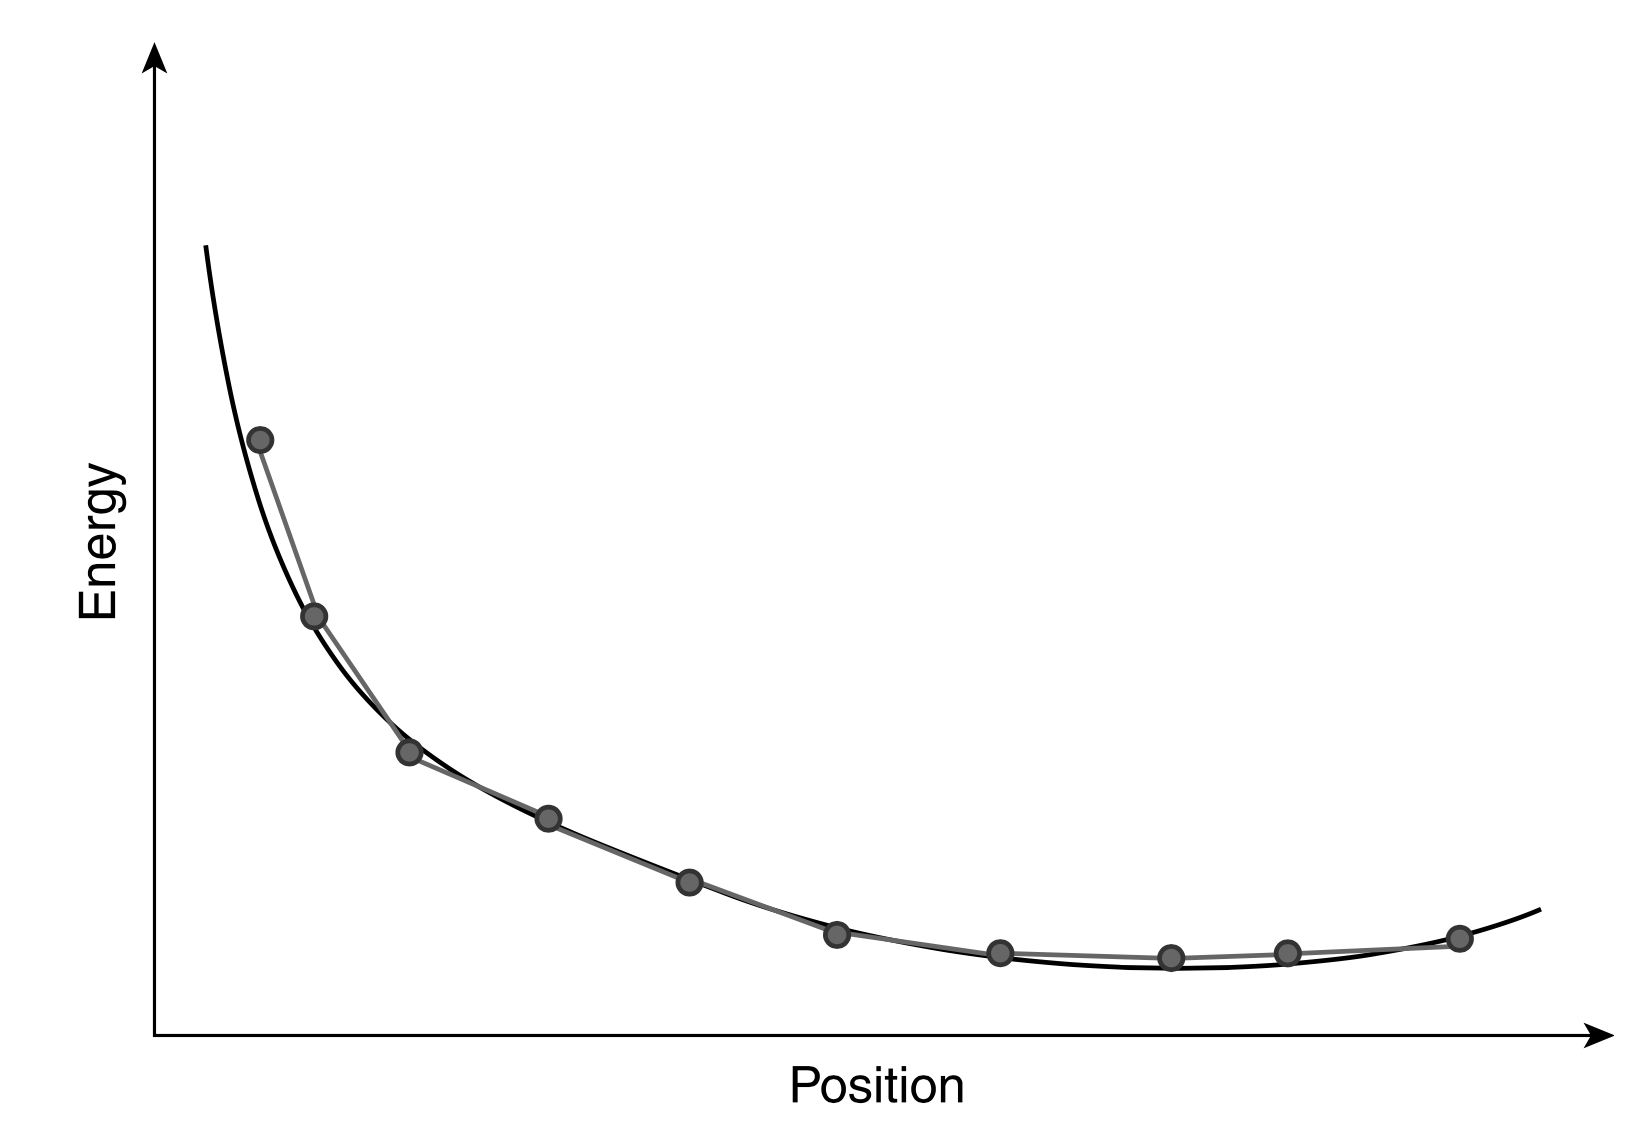
\includegraphics[width=0.5\textwidth]{practical1}
	\centering
	\caption{} 
\end{figure}

Raty et al. \cite{Raty2015} used Ab Initio Molecular Dynamics to understand the structural changes associated with aging in GeTe, and the effects those changes have on performance. Inherently out of equilibrium, amorphous materials evolve with time to a lower energetic state. In the case of phase change materials, this evolution leads to higher electrical resistivity that undermines its usability in multilevel memory devices. Using AIMD, we can watch the structure evolve, but though we discussed the addition of time to DFT above, this time is still on the order of picoseconds, leaving real-time aging out of the quesion. Raty et al. have sidestepped this problem by creating an arrangement of structures with varying local motifs. 
\par
Their study begins with the observation that AIMD simulations of Ge$_{x}$Sb$_{y}$Te$_{1+x+y}$ alloys show tetrahedrally bonded Ge (Ge$^{T}$) atoms in the amorphous phase, though these are absent in crystalline Ge. To investigate the effect of such homopolar bonds on GeTe properties, the authors melt-quenched GeTe along with a combination of other binary chalcogenides for use as``templates." SiTe forms numerous Si$^{T}$, GeSe contains some Ge$^{T}$, and SnTe contains almost no tetrahedral motifs.  The authors then substituted one species in each of the template compounds to form GeTe, i.e. substituting Si in SiTe with Ge, Se in GeSe with Te, and Sn in SnTe with Ge. After substitution, the systems were subjected to a shorter additional melt-quench procedure.
\begin{figure}[h]
	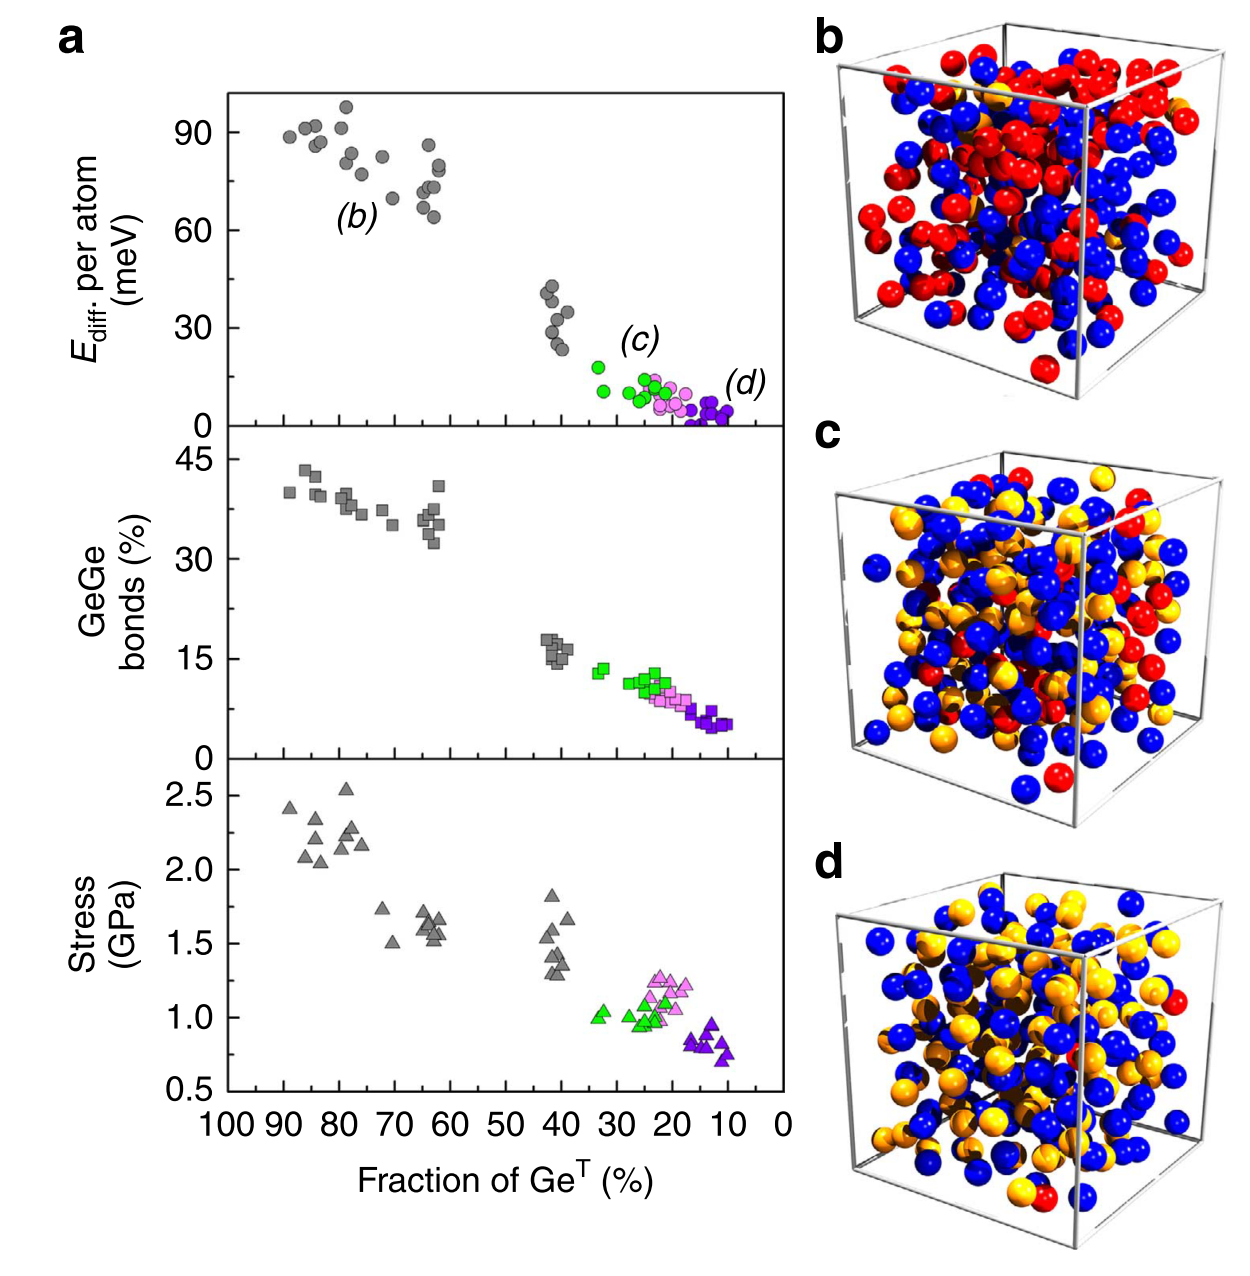
\includegraphics[width=0.5\textwidth]{raty1}
	\centering
	\caption{Results from Raty et al. \cite{Raty2015} for (a) the energy difference per atom, fraction of homopolar GeGe bonds, and stress of the melt-quenching of GeTe (green) and chemical replacement systems SnTe (violet), GeSe (pink), and SiTe (grey). (b-d) show the atomic configurations of GeTe as labeled in the energy difference plot. Te, tetrahedral Ge, and octahedral Ge are rendered in blue, red, and orange, respectively.} 
\end{figure}
\par 
The results shown in Figure. YYY indicate that the homopolar bonds reduce the stability of the system. However, homopolar bonds have a lower heat of formation in GeTe than in both GeSe and SnTe, and the melt-quench process is able to stabilize these tetrahedral motifs. In comparison to experiment, aging of phase change materials has been linked with stress relief. These results suggest that the removal of homopolar bonds contributes to this stress relief.
\par 
Raty et al. additionally calculated the changes in the electronic and optical bandgaps due to the changes in percent Ge$^{T}$. Though methods of calculating optical properties are beyond the scope of this review, the results of Raty et al. for the optical bandgap in Figures. YYY(a) and YYY show increasing band gap correlated with decreasing homopolar bonds, in agreement with experiment showing band gap widening with aging. Similarly, the DOS shows an increase in electronic band gap with aging, and the disappearance of the midgap states are directly linked to the removal of homopolar bonds. The authors note that while a variety of Ge$^T$ concentrations have been modeled, this method does not yield access to the time scale of the relaxation process. 
\begin{figure}[h]
	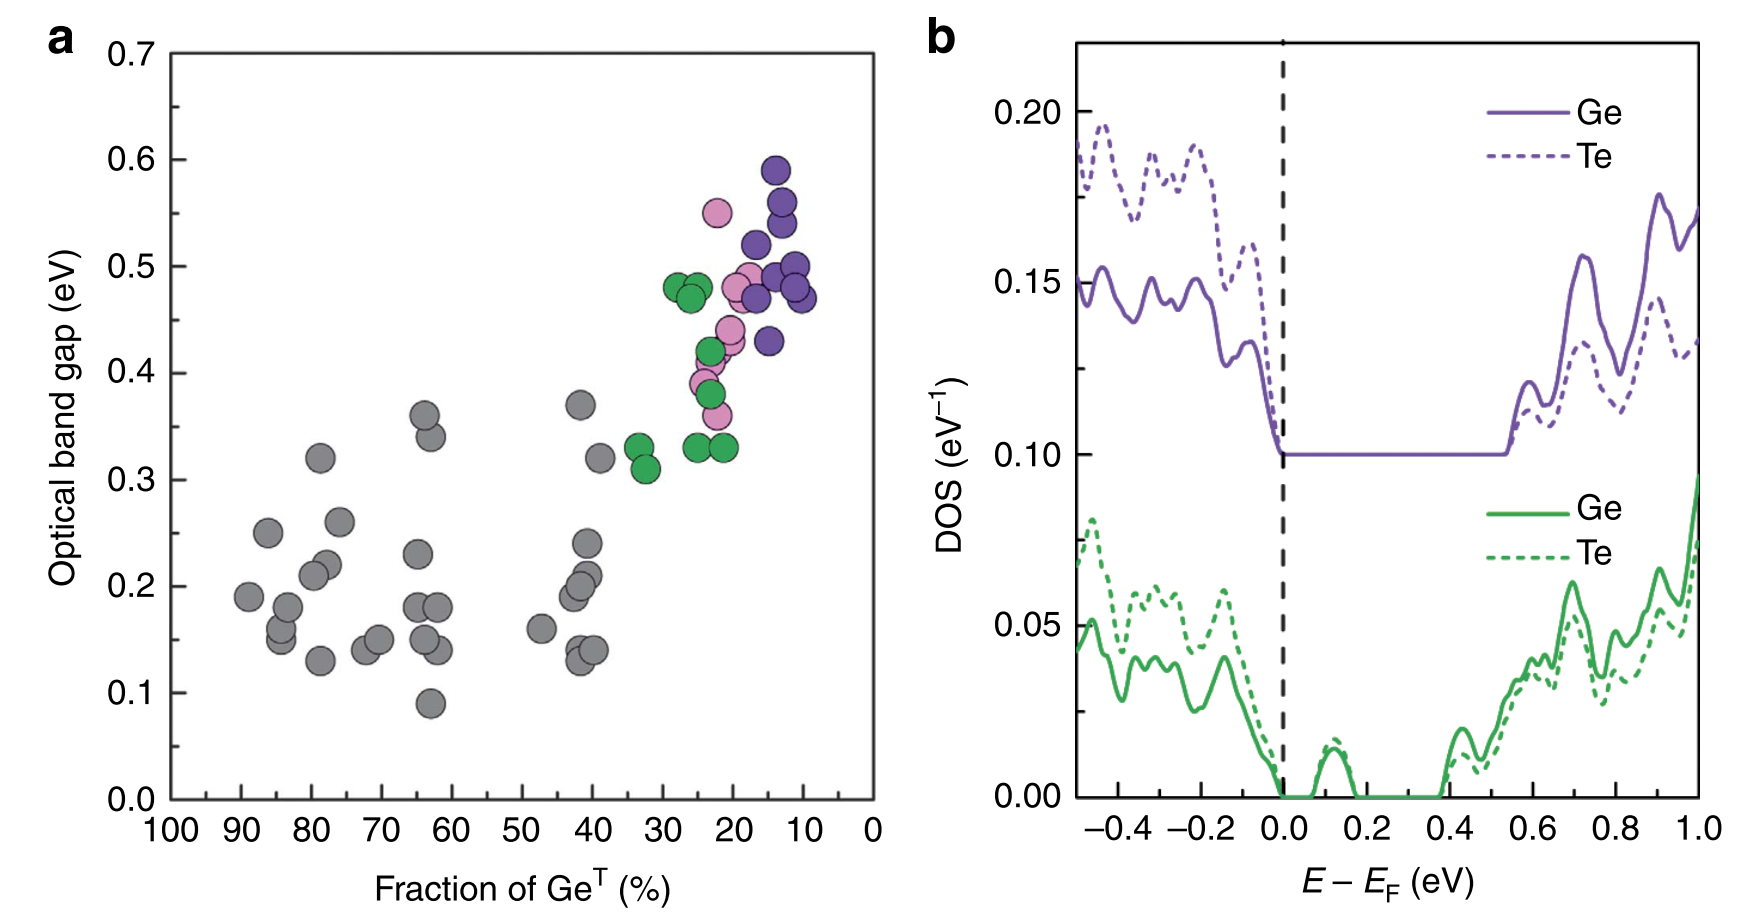
\includegraphics[width=0.5\textwidth]{raty2}
	\centering
	\caption{Results from Raty et al. \cite{Raty2015} for (a) the relaxed amorphous GeTe structures as a function of percent Ge$^{T}$} and (b) the local density of states for melt-quenched GeTe (green) and substituted a-SnTe (violet).
\end{figure}
\begin{figure}[h]
	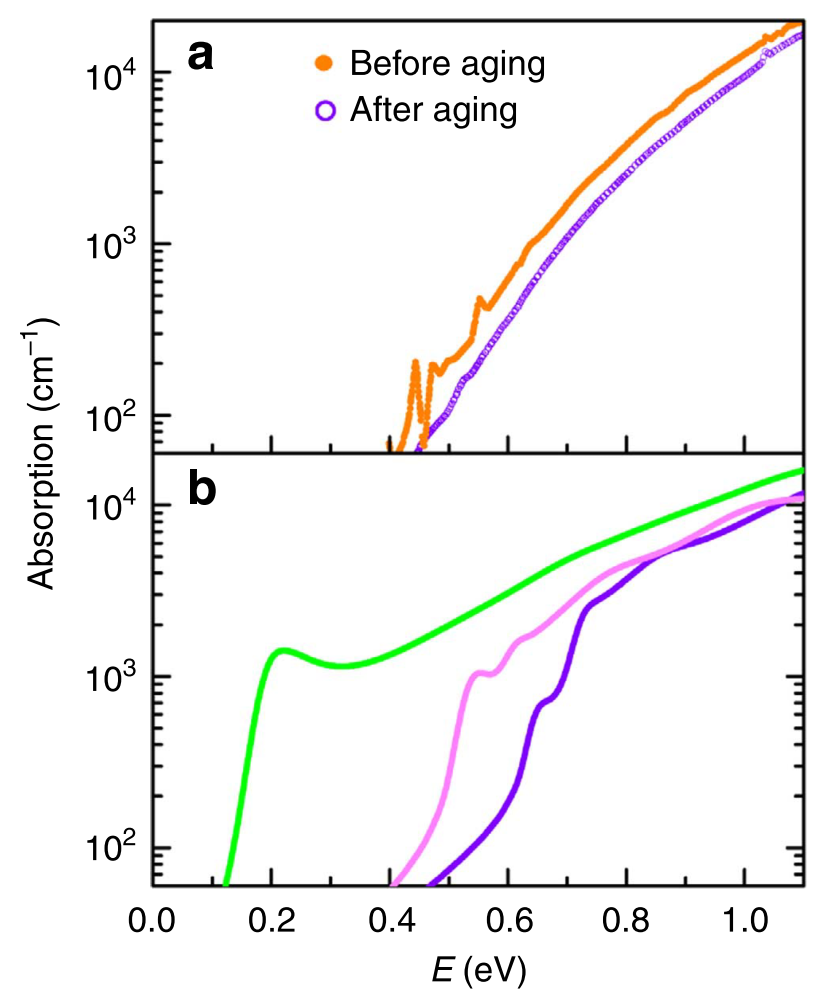
\includegraphics[width=0.3\textwidth]{raty3}
	\centering
	\caption{Results from Raty et al. \cite{Raty2015} for (a) experimental absorption from photothermal deflection spectroscopy (PDS) and (b) calculated absorption oscillator strength for melt-quenched GeTe (green), substituted a-GeSe (pink), and substituted a-Sn-Te (violet). } 
\end{figure}


\pagebreak

\section*{Notes}

\begin{itemize}
	\item Kohn Sham: A \emph{system} of one-electrons
	\item Hartree: a \emph{potential} of how each electrons feels the electron gas
	\item Hartree Fock: how we describe the wave functions
\end{itemize}
\subsection{AIMD}
\underline{Hohl 1991}\cite{Hohl1991} - Liquid and amorphous Se \par \vs
\textbf{Computational comments}
\begin{itemize}
	\item many structural models have been proposed and often conflict
	\item models based solely on small differences are insufficient to explain all measured features
	\item even carefully constructed empirical potentials have difficulty in highly anisotropic covalent systems such as group-IVA elements.
	\item AIMD avoids parameterization of interatomic forces common in MD
\end{itemize}

\underline{Raty 2015 \cite{Raty2015}} - Aging in Phase Change Materials (dots figure)
\par
\begin{itemize}
	\item Motivation
	\begin{itemize}
		\item "Amorphous materials are out of thermodynamic equilibrium"
		\item subject to physical aging
		\item phase-change materials (PCMs) have a fast, reversible switch between a conductive crystalline and more resistive amorphous phase
		\item aging increases the resistivity - `resistance drift'
		\item computer simulation to investigate relaxation processes
		\item \textbf{Modeling comment:} complexity of the chemistry requires DFT to describe and understand bonding and the amorphous phase
	\end{itemize}
	\item Literature
	\begin{itemize}
		\item DFT simulations of GeSbTe alloys report many tetrahedrally bonded Ge, which does not exist in crystal. These are obtained from MQ calcs
	\end{itemize}
	\item Methods
	\begin{itemize}
		\item Car-Parrinello
		\item \textbf{To circumvent time scale problem, generated collection of a-structures}
		\item mixed Gaussian/plane wave code in CP2K
		\item cutoff 300 Ry
		\item sampled at gamma only
		\item annealed using plane-wave code in Quantum Espresso
		\item 34 Ry
		\item 3.84 fs
		\item Berendsen thermostat
		\item 10 models produced starting from liquid
	\end{itemize}	
	\item Results
	\begin{itemize}
		\item Ge$^{T}$ is associated with homopolar Ge-Ge bonds
		\item heat of formaion shows homopolar bonds more favorable in GeTe than GeSe and SnTe
		\item wanted to investigate effects of varying amounts Ge-Ge bonds
		\item used different alloys along the phase diagram and substituted with Ge or Te to form different GeTe structures "mimicking aging"
		\item homopolar bonds correlated with tetrahedral Ge
		\item freezing at density of amorphous GeTe, tetrahedral rich models had the largest values of stress
		\item this agrees with experiments showing the drift of PCMS is accompanied by stress relief
		\item order parameter $d_{4}/d_{0}$ goes from tetrahedrally bonded Ge, $Ge^{T}$, to $Ge^{III}$ and $d_{3}/d_{0}$ goes from $Te^{II}$ to $Te^{III}$
		\item increase in band gap directly linked to decrease in homopolar bonds
		\item "melt-quenched model has a smaller band gap and possesses a (localized) mid-gap state"
	\end{itemize}	
\end{itemize}



\section*{References}

\bibliography{amorph}
\bibliographystyle{elsarticle-num}

\end{document}  